\chapter{Architettura ROS~2}
\label{chap:architettura_ros2}

Di seguito viene descritta l'architettura del sistema di controllo implementato in ROS~2, evidenziando i principali nodi e le loro interazioni. L'architettura è stata progettata per garantire modularità, scalabilità e facilità di integrazione sia con il sistema di simulazione in Unity che con il robot reale.

\section{Architettura per Unity}

L'architettura del sistema di simulazione in Unity è composta da diversi componenti principali, ognuno dei quali svolge un ruolo specifico nell'integrazione con ROS~2 e nella simulazione del comportamento del robot. I principali componenti includono:

\begin{figure}[H]
    \centering
    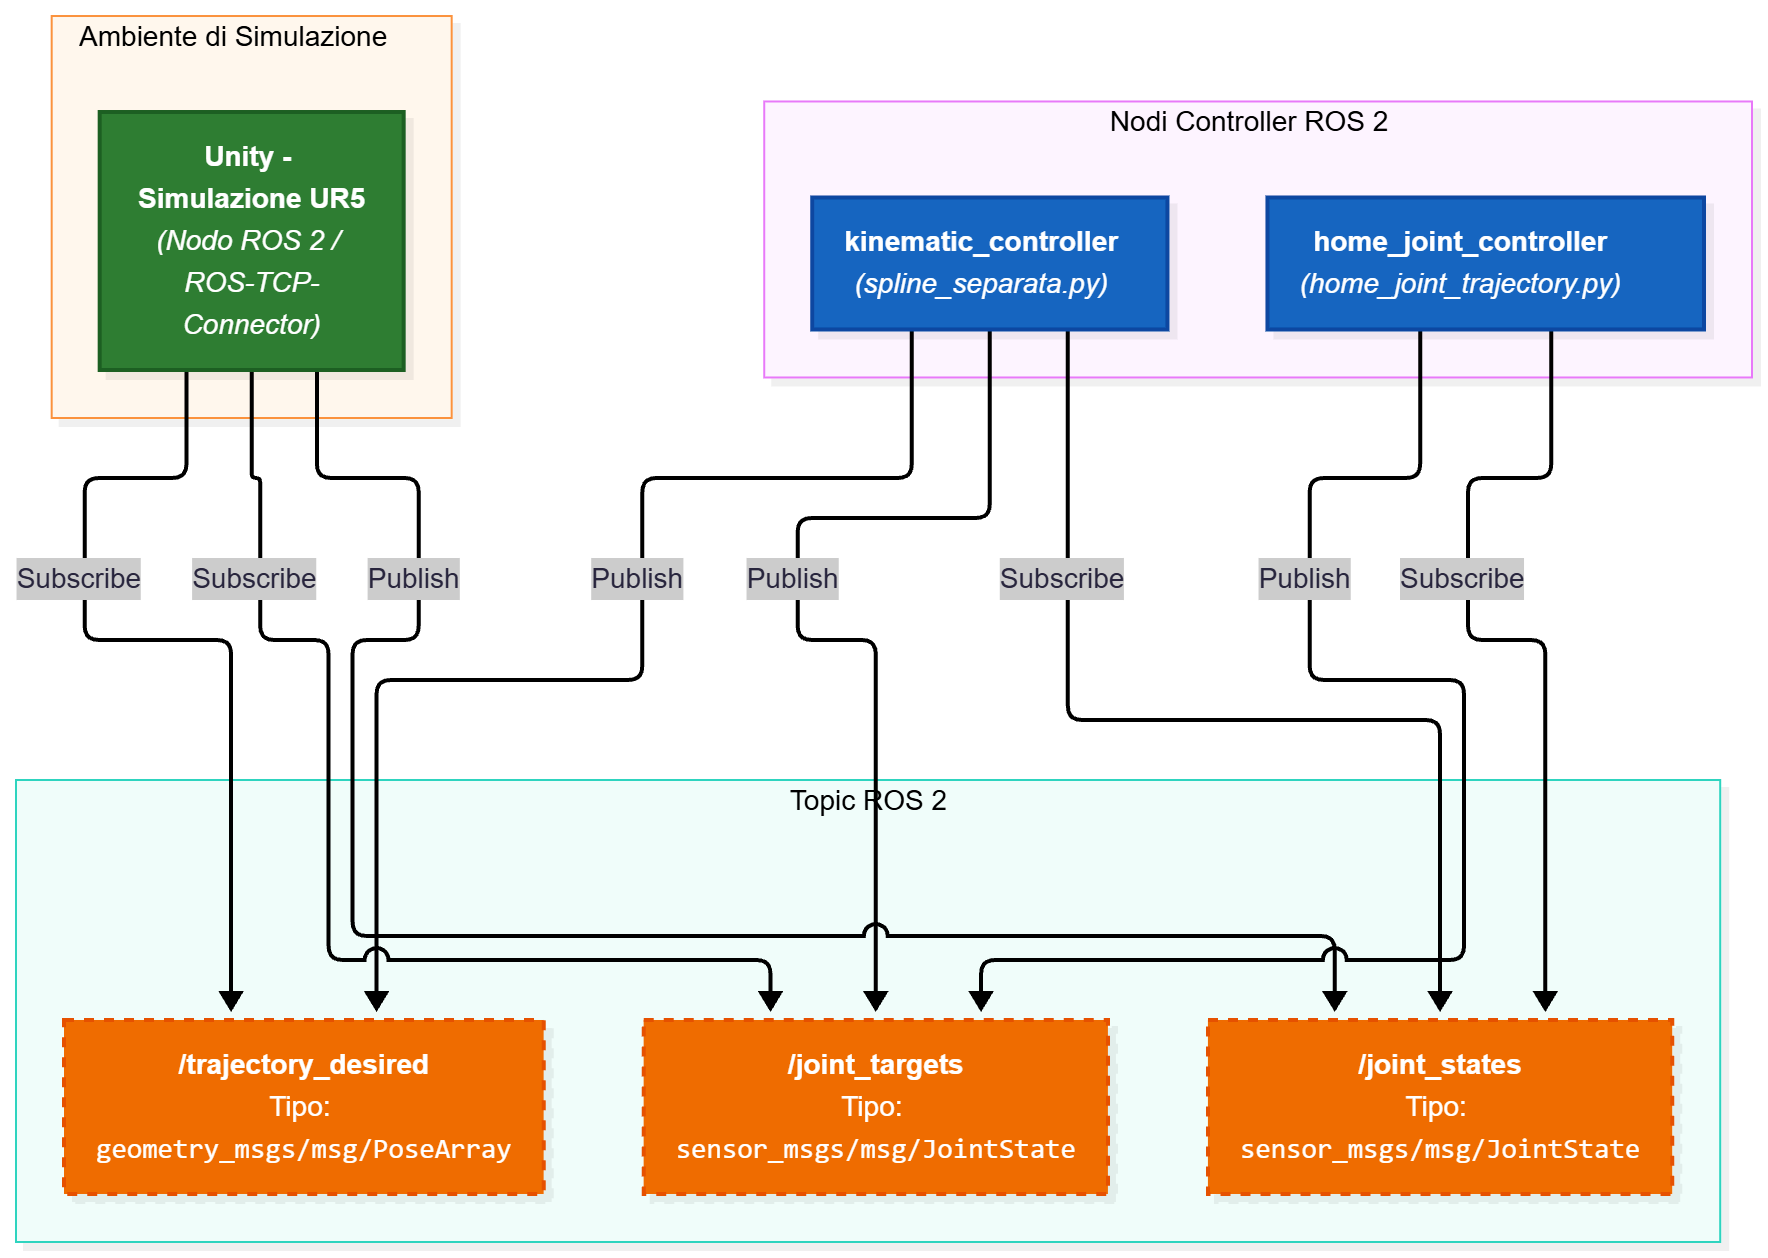
\includegraphics[width=1.0\linewidth]{figures/ros/schema_ros_unity.png}
    \caption{Architettura ROS~2 per Unity}
    \label{fig:architettura_ros2_per_unity}
\end{figure}

\newpage
\section{Architettura per il robot reale}

L'architettura del sistema di controllo per il robot reale si basa sulla struttura precedente ma con alcune modifiche per adattarsi alle specifiche del robot e alle sue capacità hardware.
Nello specifico, invece di utilizzare messaggi su topic per la comunicazione con il robot, si fa uso di action server e action client per gestire le richieste di movimento e le risposte del robot in modo più efficiente, coerentemente con il driver e controller dell'UR5.
Rispetto al caso precedente, c'è inoltre una trasformazione statica dalla camera al \texttt{wrist\_2\_link} che permette di allineare correttamente le coordinate del sistema di riferimento della camera con quelle del robot tramite poi l'utilizzo di \textit{TF}.
I principali componenti includono:

\begin{figure}[H]
    \centering
    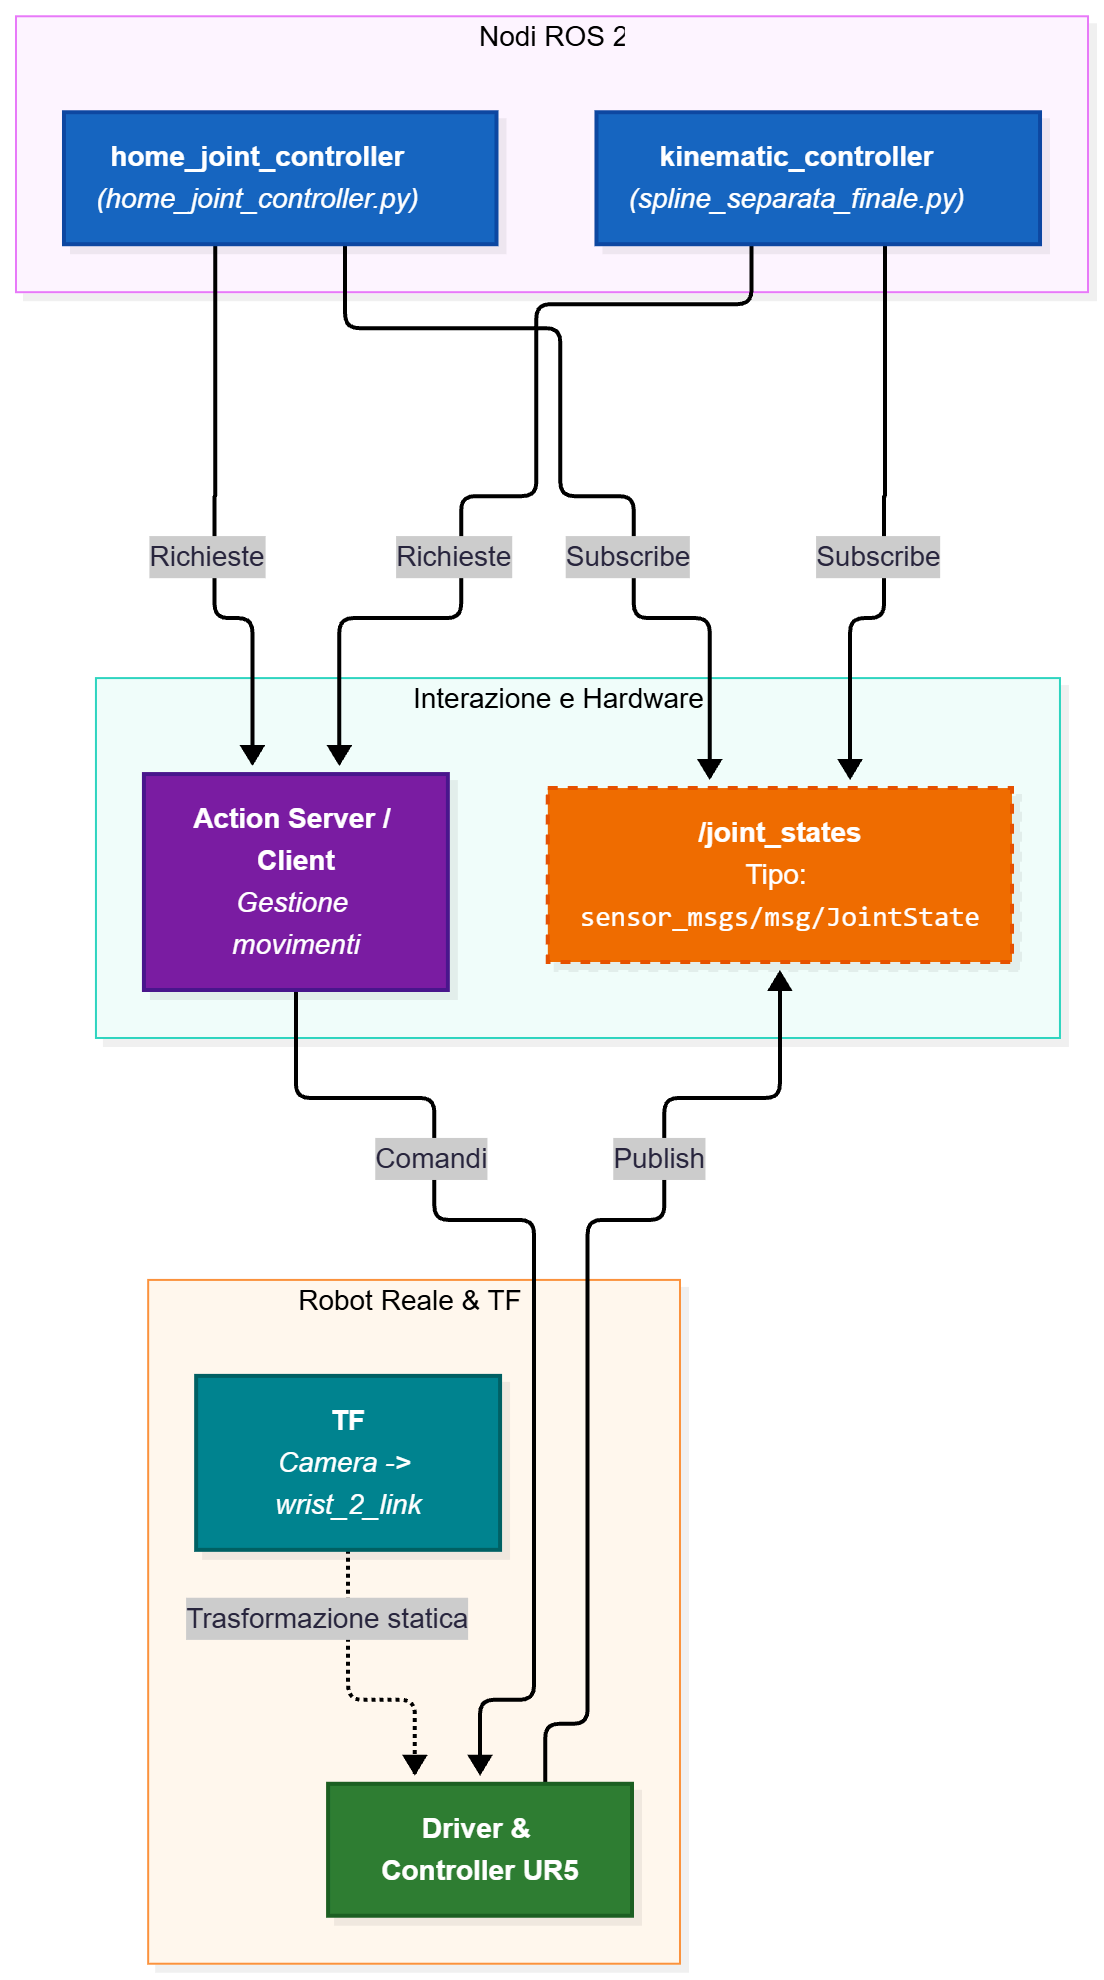
\includegraphics[width=0.5\linewidth]{figures/ros/schema_ros_reale.png}
    \caption{Architettura ROS~2 Robot reale}
    \label{fig:architettura_rosrobot_unity}
\end{figure}

\section{Architettura per il robot reale - Launcher automatico}

Questa versione dell'architettura è stata progettata per semplificare l'avvio del sistema di controllo del robot reale, automatizzando il processo di lancio dei nodi necessari e garantendo una configurazione coerente e ripetibile.
Il launcher automatico consente di avviare tutti i componenti del sistema con un singolo comando, comprendendo la traiettoria per la \textit{home\_position}, lo scatto della foto, l'inferenza del modello e la traiettoria per i punti estratti.
In questo modo si elimina la necessità di avviare manualmente ogni nodo e di riportare manualmente le coordinate dei punti estratti, riducendo il rischio di errori e migliorando l'efficienza complessiva del processo di controllo del robot.